\section{Introduction}

\STANDARD{\insertsection}
{ 
	\framesubtitle{\insertsubsection}
	
	
	\begin{itemize}
		\item This project includes use of TinyML model on an ESP32 microcontroller to digitize an analog meter
		\item Goal is to use machine learning to accurately interpret the readings of the analog meter and display them digitally
		\item Useful in monitoring energy usage or measuring the output of a device
		\item ESP32 is well-suited for this task due to its low power consumption and powerful processing capabilities
	\end{itemize}
	
	%    \begin{figure}  [!h]
		%    	\begin{center}
			%    		
\includegraphics[width=7cm]{images/Logo}
			%    		\caption{Corporacion Favorita} %\label{fig:GeneralPackages}
			%    		%{\footnotesize \textbf{Reference:} \cite{Network2020}}
			%    	\end{center}
		%    \end{figure}
	
	%\begin{figure}[!h]
	%  \centering
	%  \begin{tikzpicture}

\draw  (-3,0.5) node[left] (v1) {$q_0=q(t_0)$} ellipse (0.05 and 0.05);
\draw  (-0.5,2.5) node[right] (v2) {$q_1=q(t_1)$} ellipse (0.05 and 0.05);
\draw[-latex]  (-3,0.5) -- node[above,left]{$q=q(t)$} (-0.5,2.5);
\end{tikzpicture}
	%\end{figure}
	%  \begin{itemize}
		%    \item diese wird auch als Pose bezeichnet und kann durch 3 Positionsangaben (wie x,y,z) und 3 Drehwinkel (wie a,b,c) bezogen auf ein Bezugskoordinatensystem beschrieben werden
		%Weber, Industrieroboter Seite 16 
		%    \item sie beschreibt eine Bahn im Raum
		%  \end{itemize}  
}

\section{Challenges}

\STANDARD{\insertsection}
{ 
	\framesubtitle{\insertsubsection}
	
	
	%\textbf{Challenges}: 
	\begin{itemize} 
		\item ESP32 used for image processing in ML might be short on resources and storage.
		\begin{itemize} 
			\item Adapting the model to work with the limited resources of the microcontroller, such as memory and processing power.
			\item Optimizing the model for speed and low latency processing.
		\end{itemize}
		\item ESP32 is designed to be low-power, but running ML models can still consume a lot of power. Need to consider appropriate power source.
		\framebreak
		\item Data Acquisition and Monitoring.
		\begin{itemize} 
			\item Data Labelling and Collection ( multiple analog meters) is a time consuming activity.
			\item Data Transformation to be recognized by the ESP32 - ROI (Region Of Interest). 
		\end{itemize} 
		\item Model training is complex and computationally intensive process, particularly if you are working with a large dataset.
		\item Troubleshooting and Code Updates after Deployment.  
	\end{itemize}
	
%	\begin{figure}  [!h]
	%	\begin{center}
		%	\includegraphics[width=6cm]{images/Average monthly sales}
		%	\caption{Average monthly sales plotted} %\label{fig:GeneralPackages}
			%{\footnotesize \textbf{Reference:} \cite{Network2020}}
	%	\end{center}
%	\end{figure}
}

\section{Hardware}

\STANDARD{\insertsection}
{ 
	\framesubtitle{\insertsubsection}
	\framesubtitle{ESP32-CAM technical specifications:}
	ESP32-CAM is a small size, low power consumption camera module based on ESP32 microcontroller and OV2640 image sensor. \newline 
		\begin{itemize}
			\item 802.11b/g/n Wi-Fi SoC Module  with a speed of 2.4 GHz. 
			\item Bluetooth 4.2 with BLE. 
			\item Low-power dual-core 32-bit CPU for application processing.  
			\item Clock speed up to 160 MHz. 
			\item Computing power goes up to 600 DMIPS.
			\item Built-in 520 KB SRAM plus 4 MB PSRAM.
	\framebreak
			\item Supports Wi-Fi Image Upload.
			\item Supports multiple sleep modes.
			\item Firmware Over the Air (FOTA) upgrades are possible.
			\item 9 General-Purpose Input/Output (GPIO) ports are available.
			\item Built-in Flash LED.
			\item Supports SD card.
			\item Has an onboard PCB antenna.
			\item Has embedded Free real-time operating system (FreeRTOS) and lightweight IP.
		\end{itemize}
\pagebreak
\textbf{ESP32 CASE:}
\begin{figure}  [!h]
	\begin{center}
		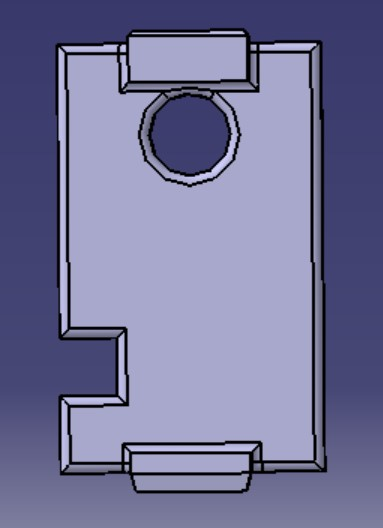
\includegraphics[width=4cm]{images/CaseTopPart}
		\caption{ESP32 Case Top Part}
	\end{center}
\end{figure}
\begin{figure}  [!h]
	\begin{center}
		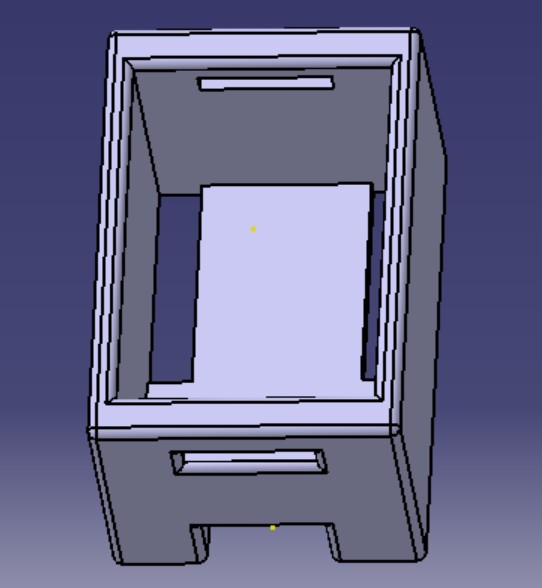
\includegraphics[width=4cm]{images/CaseBottomPart}
		\caption{ESP32 Case Bottom Part}
	\end{center}
\end{figure}
}

\section{Software}

\STANDARD{\insertsection}
{ 
	\framesubtitle{\insertsubsection}
	\framesubtitle{Visual Studio Code and Plug-in}
	Chosen IDE for the project is: VS Code: 
	\begin{itemize}
	\item VS Code is a popular and widely used integrated development environment (IDE).
	\item VS Code has a number of features that make it particularly well-suited for developing TinyML projects:
	\begin{itemize}
		\item Code completion and IntelliSense.
		\item Debugging tools.
		\item Source control integration.
	\end{itemize}
	\end{itemize}

	\begin{figure}  [!h]
		\begin{center}
			
\includegraphics[width=4cm]{images/ListMaterialvscode.jpg}
			\caption{Visual Studio Code Logo.}
		\end{center}
	\end{figure}
	
	VS Code is highly customizable and can be extended with a wide range of plugins and extensions \textbf{ESP-IDF}
	\begin{figure}  [!h]
		\begin{center}
			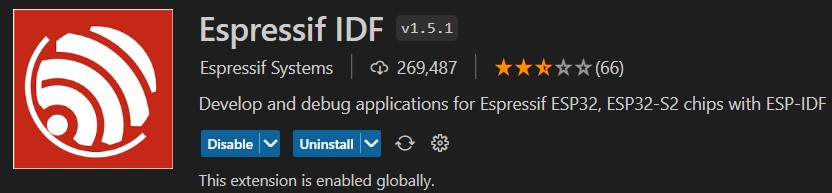
\includegraphics[width=8cm]{images/ListMaterialIDF}
			\caption{ESP-IDF Plug in in VS Code.}
		\end{center}
	\end{figure}
}

\section{Algorithm}

\STANDARD{\insertsection}
{ 
	\framesubtitle{Convolution Neural Network}
	\begin{itemize}
	\item A CNN is a type of artificial neural network specifically designed to process data with a grid-like topology, such as an image. 
	\item CNNs are preferred for image classification tasks because they are able to automatically learn and extract features from the input data, which makes them well-suited to tasks where the features of interest may not be easily defined by humans.
	\item In a digit recognition task, the input data is usually an image of a digit, and the goal is to classify the image into one of the 10 possible digits (0 through 9)
	
	\end{itemize}
To perform this task, a CNN would typically take the following steps:
\begin{itemize}
\item Preprocessing: The input image is resized and possibly normalized to a standard size and format.
	
\item Convolution: The input image is passed through one or more convolutional layers, which apply filters to the image and extract features.
	
\item Pooling: The output of the convolutional layers is passed through one or more pooling layers, which downsample the data and reduce the dimensions of the feature maps.
	
\item Classification: The output of the pooling layers is passed through one or more fully connected layers, which use the extracted features to make a prediction about the digit in the image.
\end{itemize}
\begin{figure}  [!h]
	\begin{center}
		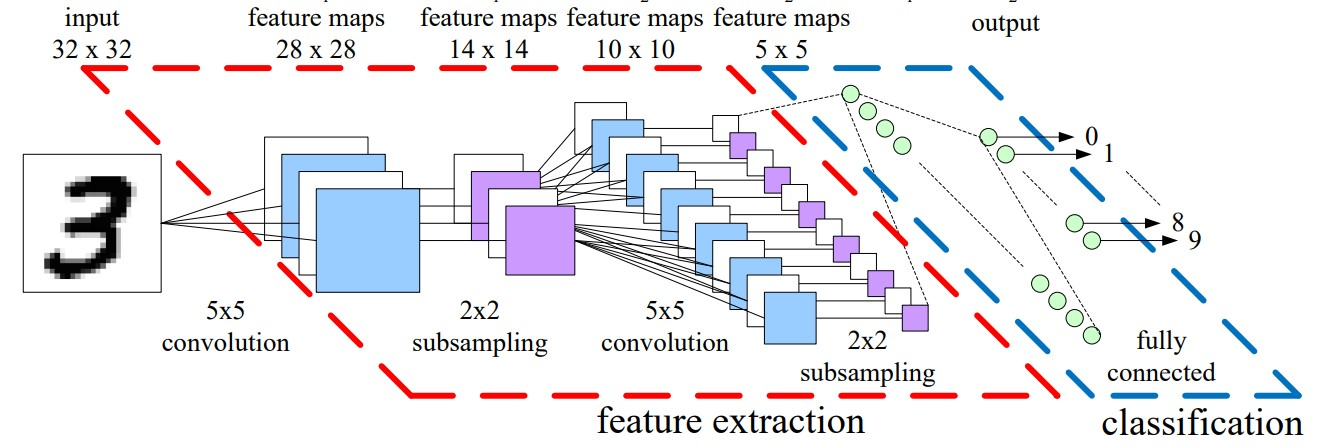
\includegraphics[width=9cm]{images/CnnLayers}
		\caption{CNN architecture for digit recognition}
	\end{center}
\end{figure}
\begin{itemize}
	\item The weights and biases of the CNN are learned through training, which involves showing the CNN a large number of labeled images of digits and adjusting the weights and biases to minimize the errors.\\
	\item Once trained, the CNN can then be used to classify new images of digits it has not seen before.
\end{itemize}
}

\section{KDD Process Implementation}

\STANDARD{\insertsection}
{ 
	
	\framesubtitle{\insertsubsection}
	\begin{itemize}
		\item Collect a dataset of images of analog meters in various states. 
		\item Preprocess by cropping and resizing the images
		\item Model training with preprocessed data
		\item Evaluate model to see how accurately it can interpret analog meter readings
		\item Model optimization to acheive desired level of accuracy
		\item Deploy the model on the device
	\end{itemize}
	
}


\section{Data Description}

\STANDARD{\insertsection}
{ 
	
	\framesubtitle{\insertsubsection}
	The dataset of images for training the model have following details:\\
	
	\begin{itemize}
		\item Before data transformation:\\
		Image size : 703 bytes - 8KB\\
		Image dimensions : 32X59 - 37X67\\
		Color space : RGB
	\end{itemize}
	
	\framesubtitle{\insertsubsection}
	\begin{itemize}
		\item After data transformation:\\
		Image size : 795 bytes - 923 bytes\\
		Image dimensions : 20X32\\
		Color space : RGB
	\end{itemize}
	

	
	
}

\section{Current Results}

\STANDARD{\insertsection}
{ 
	\framesubtitle{\insertsubsection}
	\framesubtitle{Model Generation}
		\begin{figure}  [!h]
			\begin{center}
				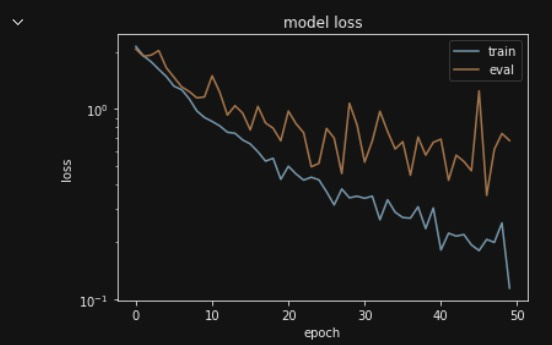
\includegraphics[width=8cm]{images/TrainedModel}
				\caption{CNN Model}
			\end{center}
		\end{figure}
	
		\begin{figure}  [!h]
		\begin{center}
			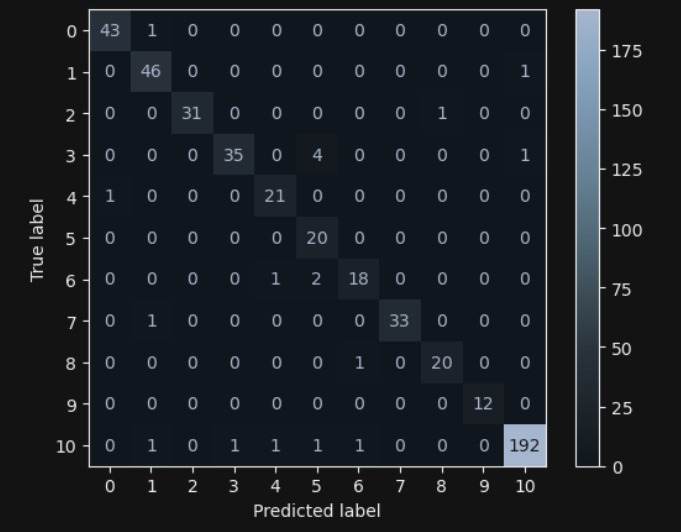
\includegraphics[width=7cm]{images/ConfusionMatrix}
			\caption{Confusion Matrix}
		\end{center}
	\end{figure}
}


\STANDARD{\insertsection}
{ 
	\framesubtitle{\insertsubsection}
	\framesubtitle{TensorFlowLite File Generation}
			\begin{figure}  [!h]
		\begin{center}
			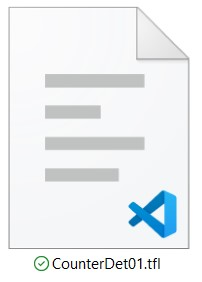
\includegraphics[width=2cm]{images/tfl.jpg}
			\caption{TnesorFlowLite Output file}
		\end{center}
	\end{figure}
}

\section{Next Steps}

\STANDARD{\insertsection}
{ 
	\framesubtitle{\insertsubsection}
\begin{itemize}
	\item Load the .tfl to ESP32-CAM.
	\item Test the model under proposed conditions. 
	\item Put the ESP32 CAM in the case for user handling.
	
		\framesubtitle{\insertsubsection}
	\begin{figure}  [!h]
		\begin{center}
			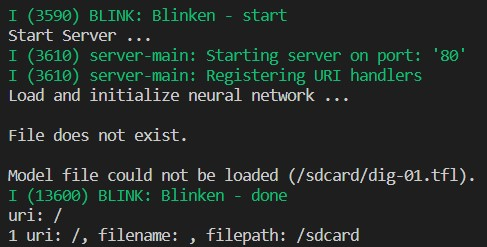
\includegraphics[width=8cm]{images/Error_tfl.jpg}
			\caption{Current Error Message to debug.}
		\end{center}
	\end{figure}
	
\end{itemize}
	
}